\documentclass[10pt,draftclsnofoot,onecolumn]{IEEEtran}
\usepackage{pdfpages}
\usepackage{lipsum}
\usepackage[utf8]{inputenc}
\usepackage[T1]{fontenc}
\usepackage{geometry}
\usepackage{setspace}
\renewcommand{\maketitle}{\bgroup\setlength{\parindent}{0pt}
\begin{flushleft}
\Huge
  \textbf{\@Multi-Camera Stereoscopic Vision: \\Requirements Document}
\large
\vspace{3mm}\\
  Erin Sullens, John Miller, Sam Schultz \\
   \vspace{3mm}
  CS461

Fall 2016

Group 54

Sponsor: Kevin McGrath

Group Name: ImMaculaTe Vision

\end{flushleft}\egroup
}
\renewcommand{\familydefault}{\sfdefault}
\usepackage[document]{ragged2e}
\geometry{letterpaper, margin=0.75in}
\newcommand\tab[1][1cm]{\hspace*{#1}}
\title{}
\author{ }

\date{October 2016}
\begin{document}
\singlespacing
%\fontfamily{lmss}\selectfont
%\begin{flushleft}
\maketitle
%\end{flushleft}
\begin{center}



\vspace{2in}
{\Medium\textbf{Abstract}
\end{center}
\setlength{\parindent}{0cm}

The requirements for the software that will be developed for Multi-Camera Stereoscopic Vision are outlined in this requirements document. We provide details about the scope of the software being created, an overall description of the requirements, and a more in-depth look at the specific requirements needed to complete this project. This document will help make the process of completing Multi-Camera Stereoscopic Vision more smoothly and will be a reference for the developers as well as our client.  \\

\vspace{.75in}
\noindent\rule{10cm}{0.4pt} \\
Kevin McGrath

\vspace{1cm}
\noindent\rule{10cm}{0.4pt} \\
John Miller

\vspace{1cm}
\noindent\rule{10cm}{0.4pt} \\
Sam Schultz

\vspace{1cm}
\noindent\rule{10cm}{0.4pt} \\
Erin Sullens
\newpage

{\Large\textbf{1 Introduction}}\\
\vspace{5mm}
{\Medium\textbf{1.1 Purpose}}\\
\vspace{5mm}
The purpose of this requirements document is to outline what the development process of Multi-camera stereoscopic vision will look like and to specify exactly how our client wants the project to function by its completion. We will cover what the software we develop will specifically do, and how any hardware we use will come into play.
 \\
\vspace{5mm}
The intended audience of this requirements document includes our client and the development team. This document will be a reference for all of us so that there is a universal understanding of what the software and hardware requirements are for this project. \\

\\
\vspace{5mm}
{\Medium\textbf{1.2 Scope}}\\
\vspace{5mm}

There will be an application for a mobile device, either Android, or iOS, and a desktop application. Both applications will take two videos as input, and do the necessary operations on them to output at video file that can be viewed in a 3D capable device. These operations include stabilizing the videos, and correlating the frames using the GPS tracking data that the cameras provide. The applications will not capture the video via real time stream from the cameras. The user will manually take the files from the cameras and transfer them to the application.

 \\
\vspace{5mm}

The benefit of developing a mobile application is that the user can start the process of combining the videos immediately after capturing the footage. The benefit of also having a desktop application is the ability to process the videos on a device that is more powerful. \\

 \\
\vspace{5mm}

{\Medium\textbf{1.3 Definitions, Acronyms, and Abbreviations}}\\
\vspace{5mm}

\textbf{1.3.1 3D capable device:}   Devices such as Google Cardboard, Samsung GearVR, HTC Vive,  Active 3D television.
 \vspace{5mm}

\textbf{1.3.2 mobile application:}   An application that can run on an Android tablet or an iPad.\\
 \vspace{5mm}
\textbf{1.3.3 desktop application:}   An application that can run on a desktop computer or a laptop, either Windows, Mac, or possibly Linux.
 \vspace{5mm}\\
\textbf{1.3.4 FPS:}   Frames per second.
 \vspace{5mm}\\
 \textbf{1.3.5 Camera:}   Garmin Camera
 \vspace{5mm}\\
 \textbf{1.3.6 FOV:}   Field of view.
 \vspace{5mm}\\
 \textbf{1.3.7 BLOB:}   Binary large object.
 \vspace{5mm}\\
 \textbf{1.3.8 Nearly simultaneously:}   Each frame of the correlated video should be no more than 16ms apart.
 \vspace{5mm}\\
 \textbf{1.3.9 FOV correction:}   The FOV of both video files should match and reflect only the section of the video that both cameras are able to see.
 \vspace{5mm}\\
 \textbf{1.3.10 Stabilized Video:}   Smoothing radius of plus or minus 30 frames

\\
\vspace{5mm}
{\Medium\textbf{1.4 References}}\\
\vspace{5mm}
NGHIAH012, 'Simple Video Stabilization Using OpenCV', 2014. [Online]. Availeble: http://nghiaho.com/?p=2093. [Accessed: 2- Nov- 2016].
\vspace{5mm}

{\Medium\textbf{1.5 Overview}}\\
\vspace{5mm}

This requirements document gives an overall view of what our Multi-Camera Stereoscopic vision project will require, in both software and hardware. It is divided into 3 main sections. Section 1 includes the purpose of this document, covers the scope of the project, and contains the definitions of some of the vocabulary used. Section 2 contains the overall description which outlines the requirements needed to create our product. Section 3 contains specific requirements where we go more in depth about the software requirements needed for our project.
\\
\vspace{5mm}

{\Large\textbf{2 Overall Description}} \\
\vspace{5mm}
{\Medium\textbf{2.1 Product Perspective}} \\
\vspace{5mm}

The desktop and mobile application is the first of its type. Currently no apps offer the ability to merge two simultaneous video files into a stereoscopic video feed for later use on a 3D capable device.\\
\vspace{5mm}
{\Medium\textbf{2.1.1 User Interfaces}} \\

\vspace{5mm}
Upload Interface: The user will have the option to upload two video files and the .FIT files for each video. They will be given the option to upload them as an entire directory or as two separate files.\\
\vspace{2mm}
			Video Browsing Interface: The user will be able to browse videos already in the system and organize them by category in user defined directories.\\
			\vspace{2mm}
Select Subset of a Video: The user will be presented with the option to download a subsection of the final converted video. The user will also have the option to select only part of the uploaded videos to be processed by the system.\\
\vspace{2mm}
Retrieval Interface: The user will have the option to choose the display device file format and download the stereoscopic video file.

\\
\vspace{5mm}
{\Medium\textbf{2.1.2 Hardware Interfaces}} \\

\vspace{5mm}
External Memory device: This will be used to download and store the final converted video.
\vspace{5mm}


{\Medium\textbf{2.1.3 Software Interfaces}} \\

\vspace{5mm}

The only software interface that our application will have at launch will consist of using our custom parser in order to convert the gps files into a workable format for the frame correlation. \\
			Name: Gps Parser\\
			Mnemonic: GP\\



\vspace{5mm}

{\Medium\textbf{2.1.4 Memory Constraints}} \\
\vspace{5mm}

Primary memory storage: The constraints on primary memory storage is determined whether the app is running on a desktop or mobile device and will restrict the initial file upload size based off device. \\\vspace{2mm}
\\
			Secondary memory storage: The converted stereoscopic video files will be stored using an external device, either cloud based storage or an external storage device.

\vspace{5mm}

{\Medium\textbf{2.1.5 Operations}} \\
\vspace{5mm}
a)User Initiated Operations: File upload, converted file retrieval\\
\vspace{2mm}
b) Interactive Operations and Unattended Operations: The user must be be able to choose what the output file format for the display device to be used. There are no unattended operations for the user.\\
\vspace{2mm}

c) Data Processing Support Functions: Support functions include video stabilization, frame syncing, GPS to frame correlation

\vspace{2mm}

d) Backup and Recovery
	The converted files will have the option to be stored on a cloud based storage service which will have its own backup and recovery routines. If the user chooses to download the converted files onto a local external storage device backup and recovery will be the user’s responsibility.


	\vspace{5mm}

	{\Medium\textbf{2.2 Product Functions}} \\
	\vspace{5mm}

	The functions of our product are: Upload two simultaneous video files, stabilize the videos, correlate the GPS data to each file, convert the two processed files into a single stereoscopic video file, retrieve converted file for use \\
		\vspace{5mm}
	{\Medium\textbf{2.3 User Characteristics}} \\
		\vspace{5mm}
Our expected user characteristics consist of a moderately educated individual who is comfortable uploading and downloading files and understands file formats. In order to meet these previous requirements, the user must have a medium level of technical expertise in order to perform the needed tasks and understand any error messages presented. \\

			\vspace{5mm}

		{\Medium\textbf{2.4 Constraints}} \\
			\vspace{5mm}
Hardware Limitations: Two identical cameras correctly mounted.\\
			\vspace{2mm}
Interfaces to other applications: Must interface with the GPS Parser (GP).\\
	\vspace{2mm}
Reliability requirements: The application must return a converted video file if the base file upload conditions are met.\\
	\vspace{2mm}
Safety and security considerations: No user will be allowed to access other users uploaded or converted videos.\\
			\vspace{5mm}
		{\Medium\textbf{2.5 Assumptions and Dependencies}} \\
					\vspace{5mm}

        The desktop application will be developed for both Windows and Mac OSX with the stretch goal of it working on certain Linux Distributions (Ubuntu, Mint, Fedora). The mobile application will be developed for Android with the stretch goal of it also working on iOS.\\
        	\vspace{2mm}
The assumptions of the application will be that the .FIT file provided by the cameras is a valid geometrics file.

        \\
        			\vspace{5mm}
{\Medium\textbf{2.6 Apportioning of Requirements}} \\
					\vspace{5mm}
{\Medium\textbf{2.6.1 Gantt Chart}} \\

        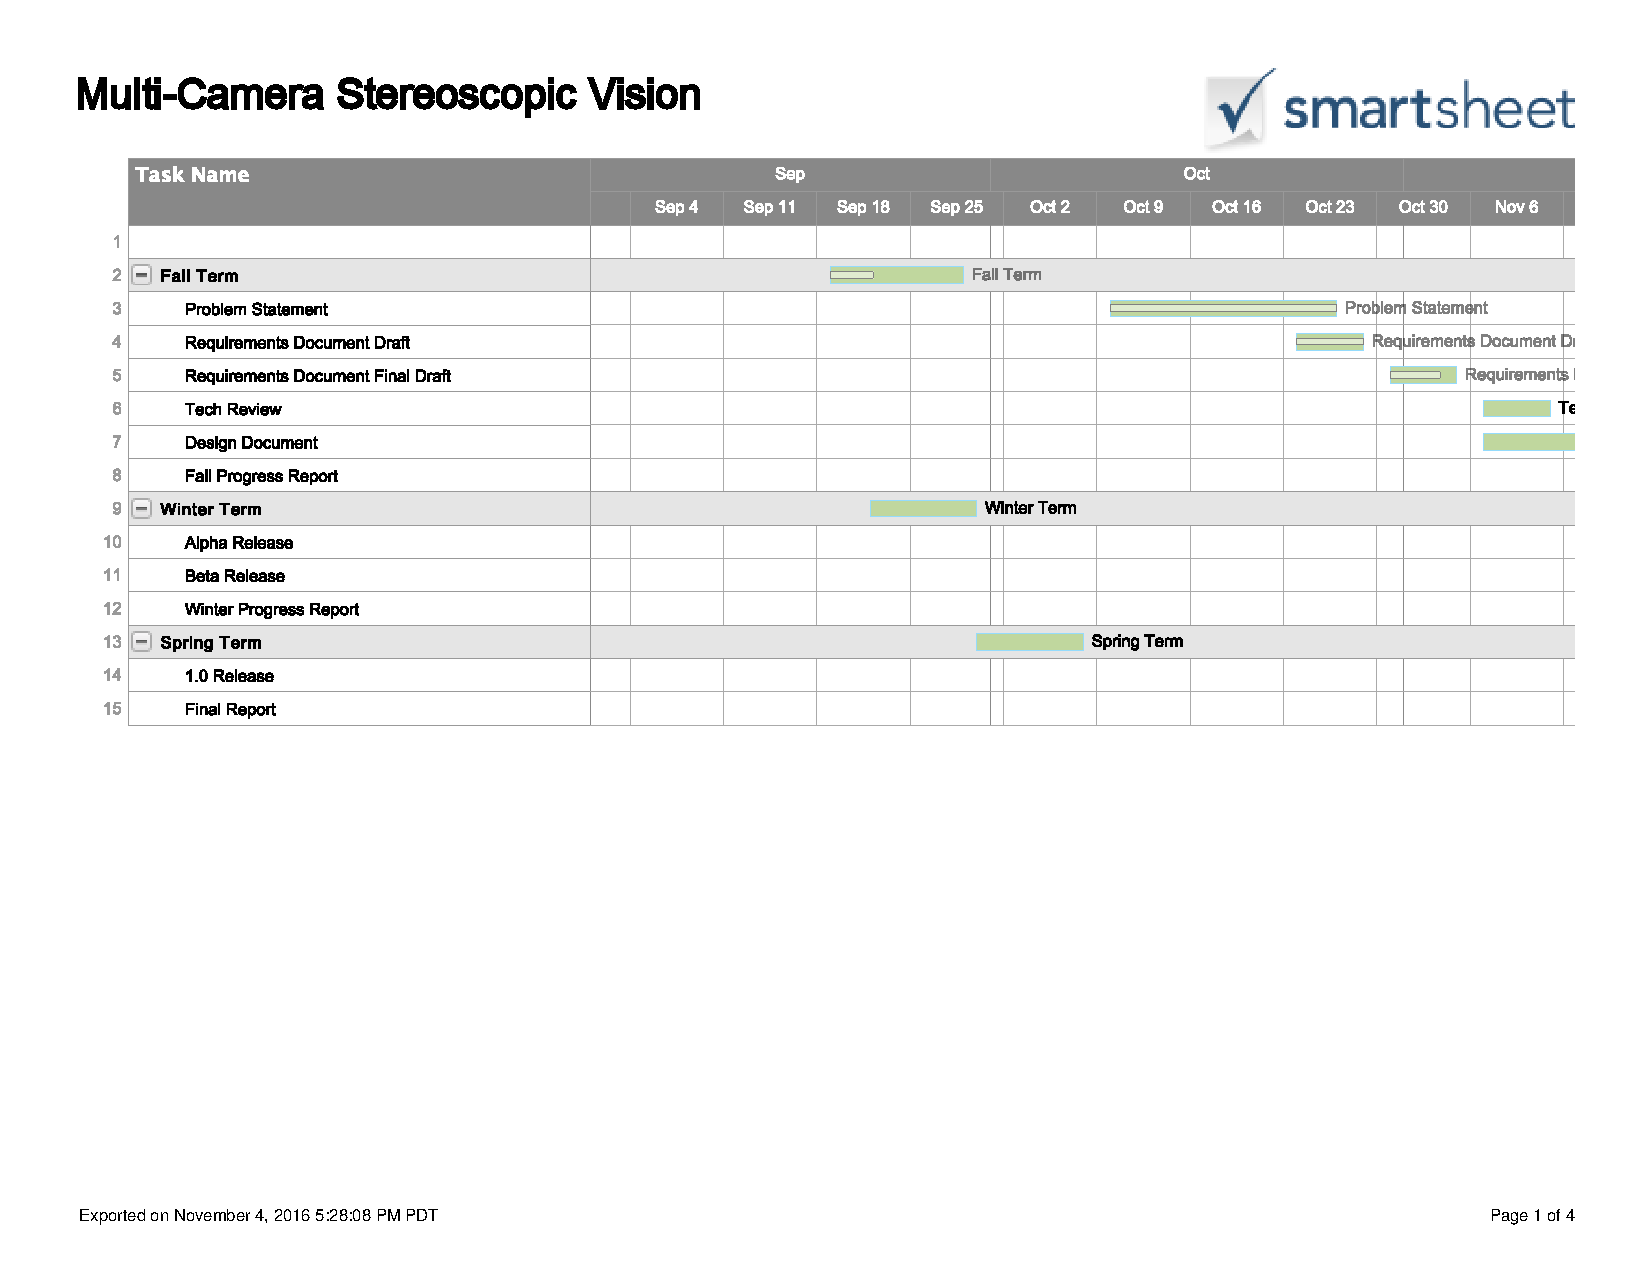
\includepdf[pages={1-3}]{rd.pdf}
        			\vspace{5mm}
{\Large\textbf{3 Specific Requirements}}\\
\vspace{5mm}
{\Medium\textbf{3.1 External Interfaces}} \\
\vspace{5mm}

The system will only have a single external interface which will be the user’s uploaded camera files (video + metadata). These will be processed and saved internally under the context of the application.\\
\vspace{2mm}


The process BLOB function will intake part of this data (the metadata), transform it, and save it either in memory or to an external file under the context of the application.\\
\vspace{2mm}


The process video file function will make use of the actual video data from the camera along with the processed BLOB data generated from the process BLOB function.\\

\vspace{5mm}
{\Medium\textbf{3.2 Functions}} \\
\vspace{5mm}
\textbf{{3.2.1 Upload Video Files}} \\
\vspace{5mm}


 The system will allow users to upload two video files along with their relevant video metadata.\\
 \vspace{5mm}
\textbf{{3.2.2 Process BLOB}} \\
\vspace{5mm}


 The cameras being used for this project output a video file in a BLOB, this process will be responsible for reading that BLOB and transforming it into a file type that our application can read. This will most likely be a JSON or CSV format. This functionality should also save this data either in memory or in a file, depending on the use case, so it can be later accessed.\\
 \vspace{5mm}
 \textbf{Validity checks on the inputs:}\\
  \vspace{5mm}

  BLOB should be in expected format
\\
 \vspace{5mm}
\textbf{Exact sequence of operations: }\\\\
 \vspace{5mm}

1. Open file pointer\\
2. Validate input file\\
3. Apply decoding algorithm to file contents\\
4. Validate Results\\

 \vspace{5mm}

\textbf{Validity checks on outputs: }\\
 \vspace{5mm}
Output file should have the following: Longitude, Latitude, Timestamp, Velocity

 \vspace{5mm}

\textbf{Responses to abnormal situations:}\\
 \vspace{5mm}
 Overflow: File too large\\
 Communication facilities: Through application provide error message to user describing the problem and what if anything they can do to remedy the situation \\
 Error handling and recovery: If possible wait for user to fix the problem otherwise cancel process\\

 \vspace{5mm}
\textbf{Relationship of outputs to inputs }\\
 \vspace{2mm}

The input of the function should contain the same data as the output, but decoded so that it is processable by the rest of our application. The output from this function feeds into the input of parses converted BLOB. \\
\vspace{5mm}

\textbf{Video Quality Assurance: }\\
 \vspace{5mm}

The system will provide video processing functionality that improves quality of given video. This should include video stabilization which follows our video stabilization requirements. \\
\vspace{5mm}

\textbf{Correlate video files: }\\
 \vspace{5mm}

The system will synchronize the two video files such that each frame are playing nearly simultaneously. This process should also involve FOV correction between the two video files. \\
\vspace{5mm}
\textbf{Convert the two processed files into a single stereoscopic video file: }\\
 \vspace{5mm}

The system will output a processed and correlated video file which can be viewed in a 3D capable device. \\
\vspace{5mm}

{\Medium\textbf{3.2.3 Parse Converted BLOB}} \\
\vspace{5mm}


 \textbf{Validity checks on the inputs:}\\
  \vspace{5mm}
Make sure decoded blob is in correct format\\
 \vspace{5mm}
\textbf{Exact sequence of operations: }\\\\
 \vspace{5mm}

1. Read decoded BLOB from file or memory\\
2. Iterate over decoded BLOB\\
3. Return specific decoded BLOB information based on request\\

 \vspace{5mm}

\textbf{Responses to abnormal situations:}\\
 \vspace{5mm}
 Overflow: If the video file is too large, the file will be cut off at 2 GB, and will start a new file containing the next frames in the sequence. \\
 Communication facilities: If running in background, push notifications. If running in foreground, on screen notifications in app. \\
 Error handling and recovery: If error is non-recoverable, report why to user. If error is recoverable prompt user to take action if necessary, otherwise attempt alternative operation

 \vspace{5mm}
\textbf{Relationship of outputs to inputs }\\
 \vspace{5mm}

Accepts decoded BLOB from Convert BLOB to parsable format function. Outputs specific metadata information about frame (e.g. gps data, frame number, etc.)
 \\\vspace{5mm}


 {\Medium\textbf{3.3 Performance Requirements}} \\
  \\\vspace{5mm}

The system should be able to process no less than 10 frames per second. This means that given 10 minutes of 60fps video, it should take no more than 60 minutes to perform all necessary operations to transform the video into the proper format.
  \\\vspace{5mm}

 {\Medium\textbf{3.4 Design Constraints}} \\
   \vspace{5mm}

 {\Medium\textbf{3.4.1 Standards Compliance}} \\
   \vspace{5mm}
   User Interface: Our application for the mobile app and desktop app should follow standard Android/iOS design requirements/best practices.
   \vspace{5mm}

 {\Medium\textbf{3.5 Software System Attributes}} \\
    \vspace{5mm}

 {\Medium\textbf{3.5.1 Reliability}} \\
Given two camera generated video files that are able to be correlated, the system should not fail.\\
 \vspace{2mm}

The system will expect the following requirements:\\
\vspace{2mm}

1. The BLOBs will be in an expected format\\
2. The two video files are capable of being correlated\\
3. Video needs to be stabilized\\
4. FOV of both cameras will be defined by the FOV camera angles of the cameras used, and will be within 5 degrees of each other. \\
5. Cameras consistent distance apart\\
6. Video taken concurrently\\

    \vspace{5mm}
 {\Medium\textbf{3.5.2 Maintainability}} \\
     \vspace{5mm}

If the BLOB format changes, the convert BLOB function should be able to change and the rest of the system remain the same. This means all functions after converted BLOB should expect and accept a consistent format.\\
    \vspace{5mm}

     {\Medium\textbf{3.5.3 Portability}} \\
     \vspace{5mm}

Mobility: The application should be usable on some mobile device (ipad, android tablet, etc.)
The underlying transformation and correlation algorithms/functions should be able to be used on any system.\\
 \vspace{2mm}
Any UI design/code should not have to be compatible with any other system unless requirements change (1 mobile, one desktop).\\
    \vspace{5mm}
 {\Large\textbf{4 Supporting Information}} \\
     \vspace{5mm}

     {\Medium\textbf{4.1 Table of Contents}} \\
          \vspace{5mm}

1. Introduction....................................................................................................................................... 2\\
          \vspace{5mm}

   \tab 1.1 Purpose................................................................................................................................ 2\\
              \vspace{5mm}

   \tab 1.2 Scope .................................................................................................................................. 2\\
                 \vspace{5mm}

   \tab 1.3 Definitions, Acronyms, and Abbreviations .......................................................................... 2\\

                 \vspace{5mm}
     \tab 1.4 References .......................................................................................................................... 2\\
                 \vspace{5mm}
    \tab 1.5 Overview ............................................................................................................................. 3\\
                 \vspace{5mm}
2. Overall Description .......................................................................................................................... 2\\
                 \vspace{5mm}

\tab  2.1 Product Perspective.............................................................................................................. 2\\
                 \vspace{5mm}



\tab\tab 2.1.1 User Interfaces........................................................................................................ 3\\
                 \vspace{5mm}
\tab\tab 2.1.2 Hardware Interfaces................................................................................................ 3\\
                 \vspace{5mm}
\tab\tab 2.1.3 Software Interfaces................................................................................................. 3\\
                 \vspace{5mm}
\tab\tab 2.1.4 Memory Constraints................................................................................................ 3\\
                 \vspace{5mm}
\tab\tab 2.1.5 Operations............................................................................................................... 3\\
                 \vspace{5mm}
\tab 2.2 Product Functions ............................................................................................................... 4\\
                 \vspace{5mm}
\tab 2.3 User Characteristics ............................................................................................................ 4\\
                 \vspace{5mm}

\tab 2.4 Constraints .......................................................................................................................... 4\\
                 \vspace{5mm}
\tab 2.5 Assumptions and Dependencies ........................................................................................ 4\\
                 \vspace{5mm}

\tab 2.6 Apportioning of Requirements ............................................................................................ 4\\
                 \vspace{5mm}

\tab\tab 2.6.1 Gantt Chart ............................................................................................................ 4\\
                 \vspace{5mm}
3 Specific Requirements ..................................................................................................................... 8\\
                 \vspace{5mm}
\tab 3.1 External Interfaces .............................................................................................................. 8\\
                 \vspace{5mm}

\tab 3.2 Functions ............................................................................................................................. 8\\
                 \vspace{5mm}

\tab \tab 3.2.1 Upload Video Files ................................................................................................ 8\\
                 \vspace{5mm}

\tab \tab 3.2.2 Process BLOB ....................................................................................................... 8\\
                 \vspace{5mm}
\tab \tab 3.2.3 Parse Converted BLOB ......................................................................................... 9\\
                 \vspace{5mm}

\tab 3.3 Performance Requirements.................................................................................................. 9\\
                 \vspace{5mm}
\tab 3.4 Design Constraints............................................................................................................... 9\\
                 \vspace{5mm}
\tab \tab 3.4.1 Standards Compliance ........................................................................................... 9\\
                 \vspace{5mm}

\tab 3.5 Software system attributes................................................................................................... 9\\
  \vspace{5mm}
\tab \tab 3.5.1 Reliability ................................................................................................................ 9\\
                 \vspace{5mm}
\tab \tab 3.5.2 Maintainability ......................................................................................................... 10\\
                 \vspace{5mm}
\tab \tab 3.5.3 Portability ................................................................................................................ 10\\
                 \vspace{5mm}
4 Supporting Information ..................................................................................................................... 10\\
                 \vspace{5mm}
\tab 4.1 Table of Contents ................................................................................................................ 10\\
                 \vspace{5mm}
\end{document}
